% -------------------- Packages --------------------

\documentclass[a4paper, oneside]{ctexbook}
\usepackage[biblatex]{packages}[2019/11/14]

% -------------------- Settings --------------------

\usepackage{pdfpages}

% Title

\title{\LaTeX 作业模板}
\author{陈旭阳}
\date{\today}

% ntheorem

\theoremstyle{nonumberplain}
\theoremheaderfont{\upshape\bfseries}
\theorembodyfont{\upshape}
\theoremseparator{.}
\theoremsymbol{}
\newtheorem{definition}{定义}

\theoremstyle{plain}
\theoremheaderfont{\upshape\bfseries}
\theorembodyfont{\itshape}
\theoremseparator{.}
\theoremsymbol{}
\newtheorem{proposition}{命题}[section]

\theoremstyle{plain}
\theoremheaderfont{\upshape\bfseries}
\theorembodyfont{\itshape}
\theoremseparator{.}
\theoremsymbol{}
\newtheorem{corollary}[proposition]{推论}

% -------------------- New commands --------------------

\newcommand{\ideal}[1]{\mathfrak{#1}}
\newcommand{\An}{\symup{A}^n}
\renewcommand{\AA}[1]{\symup{A}^{#1}}
\newcommand{\Pn}{\symup{P}^n}
\newcommand{\PP}[1]{\symup{P}^{#1}}
\newcommand{\lr}[3]{\left#1#3\right#2}

% -------------------- Document --------------------

\begin{document}
  \renewcommand{\thepage}{Cover}
  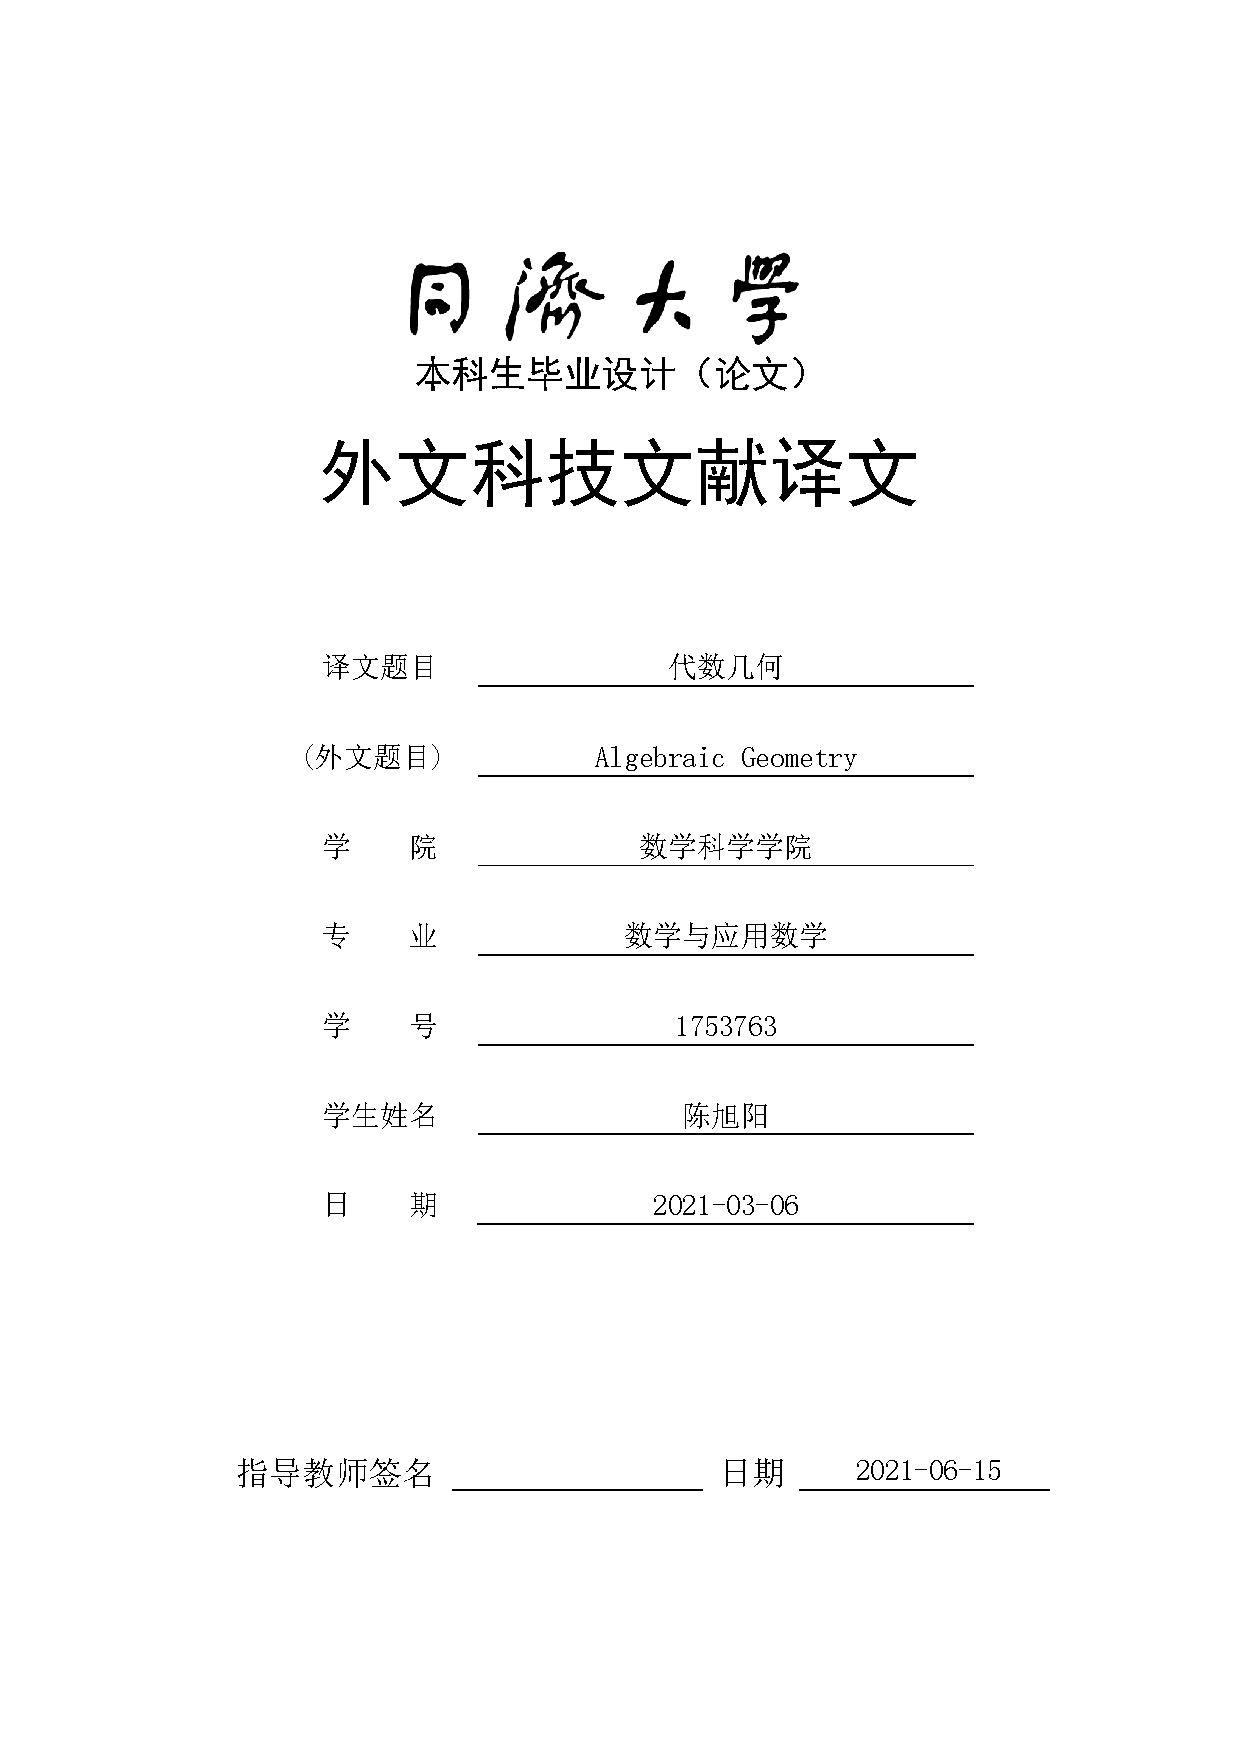
\includepdf{cover.pdf}

  \frontmatter

  \chapter{前言}

  \input{data/preface.tex}

  \chapter{介绍}

  写一本代数几何的入门书籍的困难之处在于如何在提供几何直观和例子的同时推导现代技术的语言. 对于代数几何来说, 作为学科起源的直观想法与现代研究中使用的技术方法有一道巨大的鸿沟.

首当其冲的问题就是语言. 代数几何这门学科经历了很多轮发展, 每一次都有独特的语言和看问题的观点. 十九世纪晚期代数几何有Riemann的函数论方法, 有Brill和Noether的更加几何的方法, 还有Kronecker, Dedekind和Weber的纯代数方法. 同时以Castelnuovo, Enriques和Severi为代表的意大利学派致力于代数曲面的分类. 随后二十世纪以Chow, Weil和Zariski为首的``美国"学派给意大利学派的直观提供了坚实的代数基础. 最近, Serre和Grothendieck创立了法国学派, 他们用概型和上同调的语言重写了代数几何, 并且用心的方法解决了非常多的就问题. 每一个学派都引入了很多新的概念和方法. 在写一本入门书的时候, 是用旧的语言写来贴近几何直观比较好, 还是直接从现代研究中所用的技术语言开始写比较好呢?

第二个问题是一个理念上的问题. 现代数学家倾向于抹去历史的总计: 每一个新的学派都用自己的语言重写这门学科的根基, 这样做有利于严谨性但是不利于教学. 如果一个人知道了概型的定义, 但是却没有意识到一个代数数域的整数环, 一条代数曲线和一个紧黎曼面都是一个``一维正则概型"的例子的话, 那又有什么用呢? 那么这样一本入门书籍的作者应该如何既讲明白代数几何来源于数论, 交换代数和复分析, 又给读者介绍这门学科的主要内容, 即仿射或射影空间上的代数簇, 同时推导概型和上同调这样的现代语言你呢? 有什么样的话题, 可以做到既传达代数几何的意义, 又能作为将来学习和研究的坚实基础呢?

\bigskip

我个人偏向于古典几何这一边. 我相信代数几何中最重要的问题就是那些从老派的仿射空间或射影空间的簇中引出的问题. 他们提供了激发所有后来发展的几何直观. 我以关于簇的一章开始本书, 以最简单的形式建立了一些例子和基本想法, 将它们从技术细节里解放出来. 只有在这些内容都介绍完之后, 我才能系统地建立概型, 凝聚层(coherent sheaves)以及上同调. 这些第二第三章的内容是这本书的技术核心. 在其中我试图陈述一些最重要的结论, 不过不追求一般性. 因此, 比如说上同调理论是针对N\"otherian概型上的拟凝聚层建立的, 因为这比较简单并且对于大多数应用来说已经足够强了; "顺像层(direct image sheaves)的凝聚性(coherence)"定理只证明了射影态射的情况, 并没有对一般的固有态射(proper morphism)进行证明. 因为相同的原因, 我没有引入可表函子(representable functors), 代数空间(algebraic spaces), 平展上同调(\'etale cohomology), sites以及拓扑斯(topoi)这些最抽象的概念.

第四第五章处理了古典的内容, 即非奇异的射影曲线和曲面, 但是运用了概型和上同调的技术. 我希望这些应用可以证明为了发展前两章中的技术所花费的努力是值得的.

关于代数几何的基本语言和逻辑根基, 我才用了交换代数. 它有个好处就是很精确. 并且, 通过在任意特征的域上进行研究, 我们可以获取一些基域是复数域这种古典情形下的洞见. 几年之前, 当Zariski试图编写代数几何的丛书时, 他还需要在书中自己推导需要用到的代数知识. 这项工作占据了全部工作的如此大一部分, 以致于他专门出版了一本只讲交换代数的书. 现在我们十分幸运已经有了很多出色的关于交换代数的书籍. 我关于代数的对策是在需要时引用纯代数的结论, 并给出证明的参考资料. 在书的最后列出了所有用到的代数结论.

原本我计划了完整的一系列附录 - 关于一些当今研究方向的简短介绍, 为了建立这本书的主要内容与研究的桥梁. 因为时间和篇幅有限只有三篇附录得以呈现在成书中. 我十分遗憾这本书中没能包含其余附录, 读者可以去阅读the Arcata volume, 其中有一些针对非专家的由专家所写的关于他们研究领域的文章. 此外, 关于代数几何的历史发展, 可以参考Dieudonn\'e的书. 因为没有足够多的篇幅去像我所希望的那样探索代数几何与相邻领域之间的关系, 可以参考Cassels的关于与数论关系的综述文章, 也可以参考Shafarevich的关于与复流形和拓扑的综述文章.

因为我相信主动学习是一种好的学习方法, 书中有分厂多的习题. 有一些习题包含了正文中没有介绍的重要结论. 其余习题包含了一些能阐释一般理论的具体例子. 我相信对于例子的研究与发展一般理论之间有着不可分割的关系. 认真的学生应该尝试尽可能多地做这些习题, 但是不应该觉得能立即解出他们. 有不少习题需要一些真正有创造性的努力才能够理解. 一个星号表示这道习题是困难的, 两个星号表示这道习题是一个未解决的问题.

(I, \S 8)中有关于代数几何和这本书的进一步介绍.

\subsection*{术语}

大部分情况, 书中的属于与广泛接受的用法是相同的, 不过还是有一些值得注意的例外. \emph{簇}一直是不可约的, 并且一直是在代数闭域上的. 在第一张中所有的簇都是拟仿射的. 在(II, \S 4)中簇的定义被拓展为包括\emph{抽象簇}, 即为代数闭域上的integral separated schemes of finite type, 词语\emph{曲线}, \emph{曲面}和\emph{3-fold}分别用来表示1维, 2维和3维的簇. 但是在第四章中, 词语\emph{曲线}只用来表示非奇异的射影曲线; 在第五章中\emph{曲线}表示任何非奇异射影曲面上的有效除子(effective divisor). 第五章中\emph{曲面}表示非奇异射影曲面.

书中的\emph{概型}在第一版的EGA中被称为预概型(prescheme), 不过在新版EGA中被称为概型.

书中\emph{射影态射}和\emph{very ample invertible sheaf}的定义与EGA中的定义并不等价. 他们在技术上比较简单, 但是有一个缺点就是它并不是基上的局部概念. 词语\emph{非奇异}只对簇使用, 对于一般的概型来说, 我们采用\emph{正则}和\emph{光滑}.

\subsection*{代数的结论}

我假设读者熟悉环, 理想, 模, N\"otherian环, 整相关(integral dependence)的基础知识, 并且乐意接受或者查询其它属于交换代数或者同调代数结论, 这些结论如果需要的话会在书中进行陈述, 伴有相关文本的引用. 这些结论会被标注一个A, 比如说定理3.9A, 为了和书中证明的结论进行区分.

基本的约定有这些: 所有的环都是交换幺环, 单位元记作1. 所有的环同态都将1映到1. 在整环或者域中, $0\neq 1$. 一个\emph{素理想}(或者极大理想)是环$A$的一个理想$\ideal{p}$, 满足商环$A/\ideal{p}$是一个整环(或者域). 因此环本身不被认为是一个素理想或者是极大理想.

环$A$中的一个\emph{乘性系统}(multiplicative system)是一个包含1的子集$S$, 满足关于乘法封闭. \emph{局部化}$S^{-1}A$定义为分式$a/s, a\in A, s\in S$在等价关系下的商, 其中$a/s$与$a'/s'$\emph{等价}仅当存在$s''\in S$使得$s''(s'a-sa')=0$成立. 有两种一直用的局部化列举如下. 设$\ideal{p}$是$A$中的素理想, 那么$S = A - \ideal{p}$是一个乘性系统, 相对应的局部化被记为$A_{\ideal{p}}$. 如果$f$是$A$的元素, 那么$S = \{1\}\cup \{f^n\vert n\geq 1\}$是一个乘性系统, 相对应的局部化被记为$A_f$. (注意在$f$是幂零元的情况下, $A_f$是零环.)

\subsection*{引用}

关于定理, 命题, 引理的交叉引用用圆括号以及数字, 例如(3.5). 对习题的引用例如(习题3.5). 对另一章节的结论的引用以章节数字打头, 例如(II, 3.5)或(II, 习题3.5)


  \mainmatter
  \renewcommand{\thechapter}{\Roman{chapter}}
  \renewcommand{\thesection}{\arabic{section}}
  \chapter{簇}

  \input{data/chap01.tex}

  \clearpage
  \pagenumbering{arabic}
  \renewcommand{\thepage}{O\arabic{page}}
  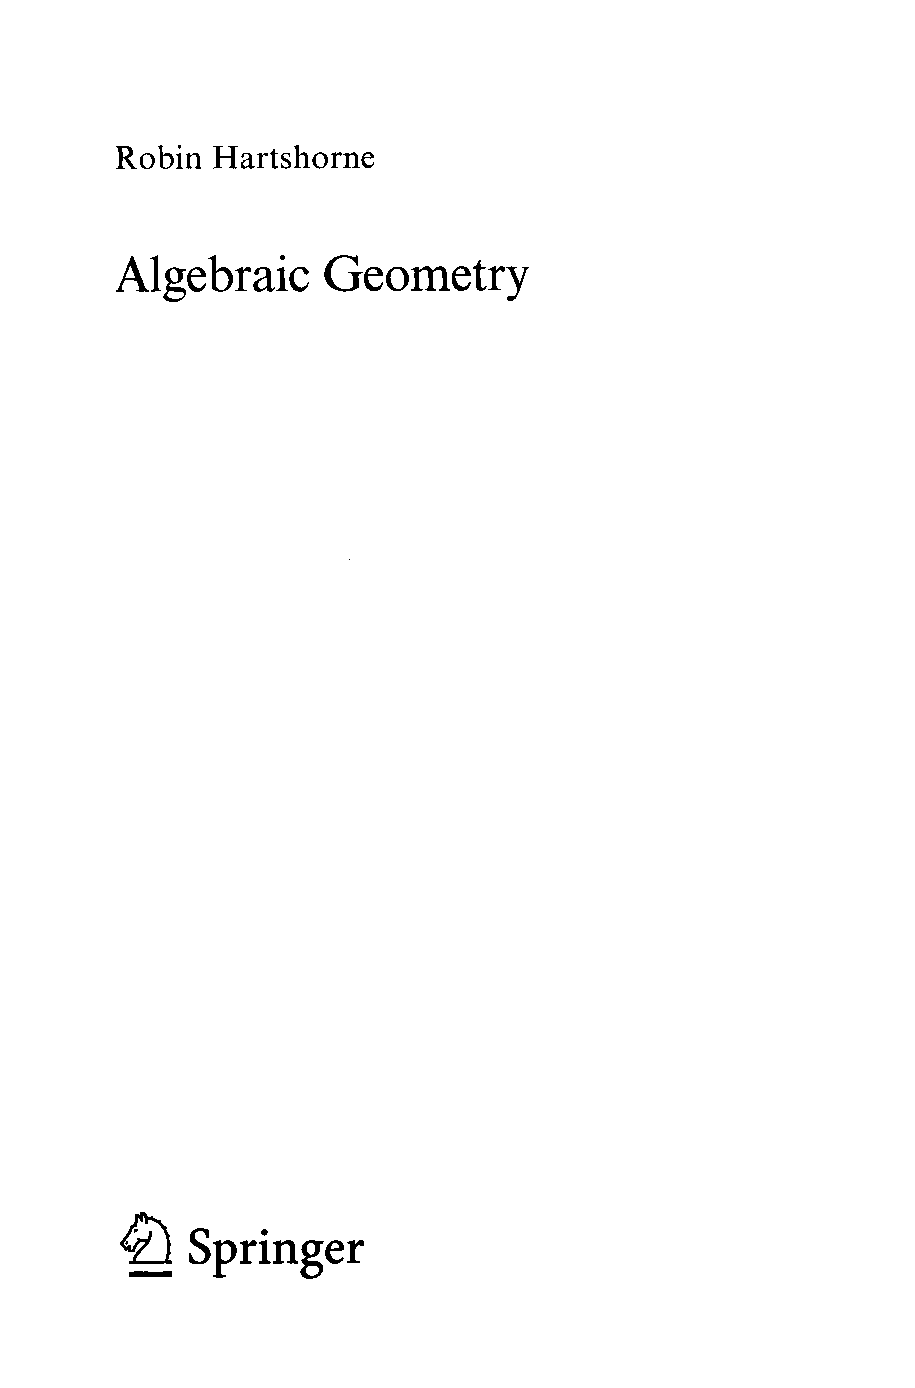
\includepdf[pages=-]{origin.pdf}

\end{document}
